\chapter{\cpserver{} Design}
\label{chap:cpserver}

To demonstrate the benefits of \cphash{} in an application we developed, \cpserver{}, a memcached style
Key/Value Cache Server, which uses \cphash{} to implement its hash table.
\cpserver{} has server and client threads as described in Chapter \ref{chap:mcstore}; however,
it also has clients that connect to the server using TCP connections. To avoid confusion with names of client threads and
clients that connect over TCP, we will call the latter TCP clients. Figure \ref{fig:mcserver} shows the design of \cpserver{}.

The server threads operate as described in Chapter \ref{chap:mcstore}. Client threads monitor TCP connections assigned to them 
and gather as many requests as possible to perform them in a single batch. Then, as described in Chapter \ref{chap:mcstore}, client threads pass the 
requests to the appropriate server threads using message passing. After the server threads are done and the client threads receive their results back, they write back 
those results to the appropriate TCP connections. 

The \cpserver{} also has a TCP server thread that accepts new connections. When a connection is made, 
it is assigned to a client thread with the smallest number of current active connections. For our testing needs this simple type of load balancing works fine, 
however the load balancer could be more advanced for work loads in which the traffic on different connections differ significantly.


\begin{figure}[!ht]
  \centering
  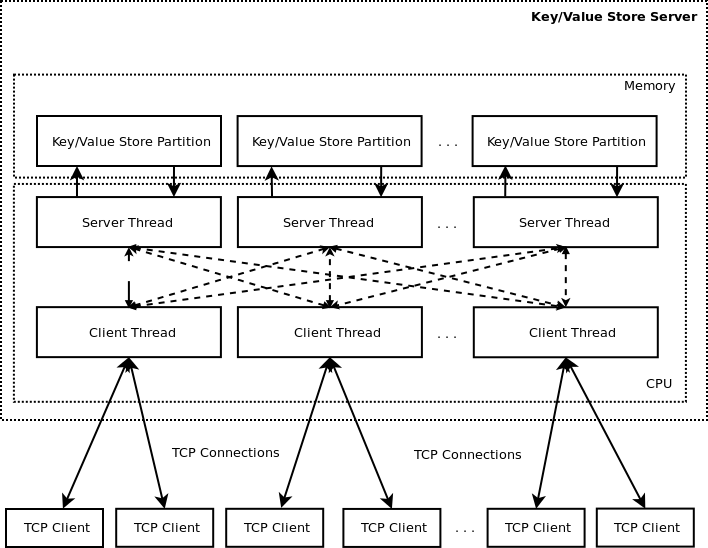
\includegraphics[width=1.0\linewidth]{figs/mcserver.png}
  \caption{\cpserver{} design}
  \label{fig:mcserver}
\end{figure}

\section{Protocol}

\cpserver{} uses a simple binary protocol. Figure \ref{fig:protocolrequest} presents binary format of a request header.
Figure \ref{fig:protocolresponse} present binary format of a response.

\begin{figure}[!ht]
  \centering
  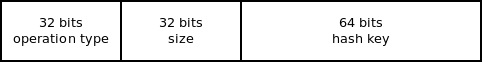
\includegraphics[width=0.8\linewidth]{figs/protocolrequest.png}
  \caption{\cpserver{} request header}
  \label{fig:protocolrequest}
\end{figure}

Two operation types currently supported are: LOOKUP and INSERT.
\begin{description}
\item[LOOKUP] With the LOOKUP request the TCP client asks the server to try to find a key/value pair in the hash table
such that the key matches the \texttt{hash key} field from the request. The \texttt{size} field is unused for the LOOKUP request,
thus it can be set to any value.
\item[INSERT] With the INSERT request the TCP client asks the server to insert a new key/value pair in the hash table. 
The \texttt{hash key} field is the key to be inserted. The \texttt{size} field is the size of the value to be inserted in the hash table.
The INSERT request header is followed by \texttt{size} amount of bytes which describe the value to be inserted.
\end{description}

The actual supported size of the hash key in \cphash{} is 60 bits, thus the most significant 
4 bits of the \texttt{hash key} field will always be ignored by the server.

\begin{figure}[!ht]
  \centering
  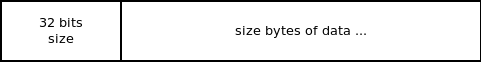
\includegraphics[width=0.8\linewidth]{figs/protocolresponse.png}
  \caption{\cpserver{} response}
  \label{fig:protocolresponse}
\end{figure}

The responses for currently supported operations are the following:
\begin{description}
\item[LOOKUP] For the LOOKUP requests, if a key/value pair is found in the hash table such that the key matches
the \texttt{hash key} provided in the LOOKUP request, then the size of the value and the actual value data are returned.
Otherwise if such a key/value pair can not be found in the hash table, a response with a \texttt{size} of 0 is
returned.
\item[INSERT] The INSERT requests are silent, thus for them there is no response returned from the server.
\end{description}

\section{Handling Any Size Keys}
\label{sec:anykey}

In our current implementation only 60 bit hash keys are supported. This can easily be extended to any size keys
without modifying \cpserver{}. The main idea to support any size keys is to use the 60 bit hash of the given any size key as a hash key and store both the 
key and the value together as a value. Then to perform the LOOKUP of a certain key, we would first calculate the hash key
and lookup the value associated with it. If such a value exists it would contain both the key string and the value string in
it. Then before returning the value we would compare the key string to the actual key that we wanted to lookup and if
return the value. If the key strings do not match, this would mean we got hash collision since their hash values match but the 
strings itself do not. In this case we would just return that the value was not found. The chance of collision with 60 bit keys 
would be very small, especially considering the fact that the hash table is stored in memory thus it can not have more than 
couple billion elements in it.

To perform the INSERT operation we would calculate the hash key from the key string and insert a key/value pair in the hash table
where the key would be our calculated hash key and the value would be a combined string of both the key and the value.

